\chapter{Digráficas de intervalos ajustadas}
\label{cap:DigrafIntAj}

\section{Digr\'aficas de intervalos}

En el año 1989 se publicó un articulo de M. Sen, S. Das, A.B. Roy y D.B. West en el  \textit{Journal of Graph Theory}. En este se introduce una nueva definición que generaliza a las gráficas de intervalos. Dicha generalización iba enfocada a tener caracterizaciones análogas a las de las gráficas de intervalos, una de ellas, la propiedad de los unos consecutivos para columnas de la matriz asociada a la gráfica de clanes maximales. 
Desafortunadamente esta definición, no cuenta con un alguna caracterización en términos de estructuras prohibidas, como sí las tienen las gráficas de intervalos, en términos de las tripletas asteroidales y $k$-ciclos sin cuerdas, $k \geq 4$. Así, al solo contar con una caracterización sencilla, a saber, a través de la propiedad de los unos consecutivos, el único algoritmo de reconocimiento para esta clase no es eficiente.

En el artículo arriba mencionado, se define una digráfica de intervalos como una digráfica $G$ la cual admite una representación de pares de intervalos, es decir, para cada vértice $v \in V(G)$, existen $I_v,J_v$ un par de intervalos, y $uv\in E(G)$ si y solo si $I_u$ intersecta a $J_v$. 

En el ánimo de explorar las propiedades de las digráficas de intervalos surge una pregunta muy natural. ¿Puede una digráfica, cuya gráfica subyacente no sea una gráfica de intervalos, ser una digráfica de intervalos? La respuesta puede responderse inmediatamente mediante este primer ejemplo. Comencemos con una digráfica muy sencilla, la cual se muestra en \cref{fig:Dgrf01} y consta únicamente de dos vértices, $v_1, v_2$, y que carece de flechas, así como de lazos. Una representación por pares de intervalos se muestra en la parte inferior, y es fácil comprobar que las incidencias se respetan, pues los cuatro intervalos son ajenos dos a dos. Pero en particular $I_1$ no intersecta a $J_1$ ni a $J_2$ e $I_2$ tampoco intersecta a $J_1$ o a $J_2$. Para responder la pregunta, hacemos la siguiente nota, en la definición de las gráficas de intervalos es implícito que las gráficas cuenten con lazos, mas aún que sean reflexivas. Como primer contraste, en el caso dirigido se pierde esto, como se mostró en el presente ejemplo. Así que el hecho de que la gráfica suyacente no sea gráfica de intervalos no nos arroja mayor información. 

\begin{figure}[H]
  \centering
  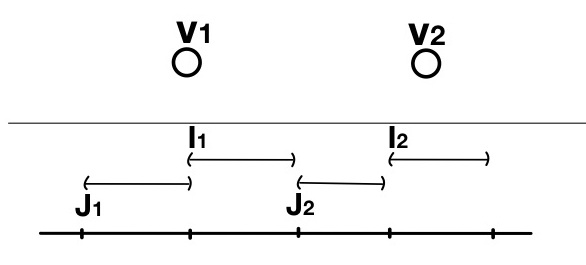
\includegraphics[width=0.5\textwidth]{recursos/capturas/Digraf1.jpg}
  \caption{Digráfica sin flechas ni lazos.}
  \label{fig:Dgrf01}
\end{figure}


Ahora vemos que al añadir una flecha que sale de $v_1$ a $v_2$ nosotros seguimos teniendo que esta digráfica tiene una representación por pares de intervalos. Para dar la representación, podemos usar como base la que se dio en la imagen anterior y solo modificar los intervalos $I_1,J_2$; debemos buscar que $I_1\cap J_2 \neq \emptyset$, es decir, que tengan intersección no vacía, ya que queremos rescatar el hecho de tener la flecha $(v_1,v_2)$. Para lograr esto, basta extender un poco hacia la derecha el extremo derecho del intervalo $I_1$. 

\begin{figure}[H]
  \centering
  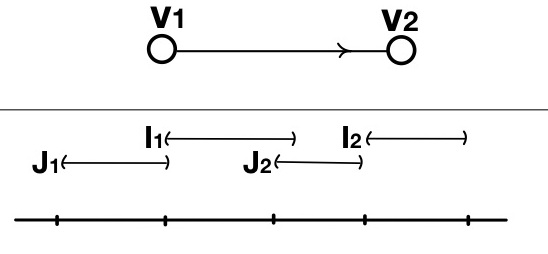
\includegraphics[width=0.5\textwidth]{recursos/capturas/Digraf2.jpg}
  \caption{Digráfica con una sola flecha.}
  \label{fig:Dgrf02}
\end{figure}


A continuación en \cref{fig:Dgrf03} se muestra que al añadir la flecha en el otro sentido se sigue teniendo una representación de pares de intervalos y por tanto se tiene que nuevamente es digráfica de intervalos. Para verificar esto, comenzamos haciendo una pequeña modificación a la representación de pares de la figura anterior. En primer lugar situamos el intervalo $I_2$ a la izquierda de todos los intervalos y extendemos el extremo derecho del intervalo de tal forma que este intersecte al intervalo $J_1$.

\begin{figure}[H]
  \centering
  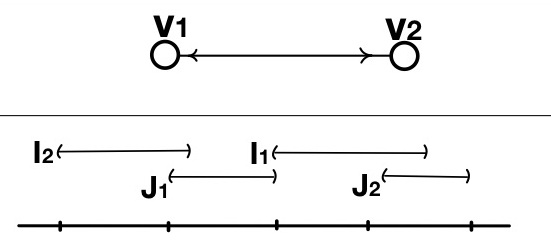
\includegraphics[width=0.5\textwidth]{recursos/capturas/Digraf3.jpg}
  \caption{Digráfica con dos flechas.}
  \label{fig:Dgrf03}
\end{figure}

Finalmente exhibimos que al añadir todas las posibles flechas y lazos en el ejemplo dado en \cref{fig:Dgrf01} seguimos teniendo una digráfica de intervalos. Tomamos la representación del ejemplo anterior y para añadir el lazo en $v_1$ tenemos que $I_1$ debe intersecar a $J_1$ y análogamente tenemos que hacer que $I_2$ intersecte a $J_2$ para así tener el lazo en $v_2$. Notese que $I_1$ e $I_2$ pueden o no intersectarse pues esto no afecta a las flechas, aquí los ponemos disjuntos.

\begin{figure}[H]
  \centering
  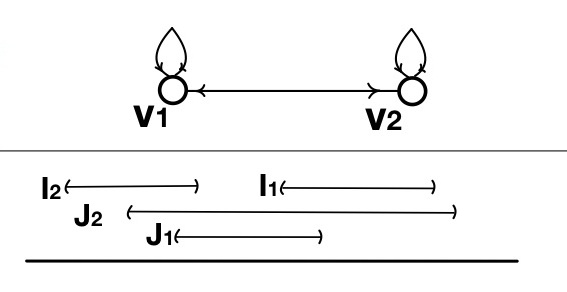
\includegraphics[width=0.5\textwidth]{recursos/capturas/Digraf4.jpg}
  \caption{Digráfica de dos vértices y todas las flechas y lazos posibles.}
  \label{fig:Dgrf04}
\end{figure}
 
Como se vio desde nuestro primer ejemplo, una digráfica de intervalos puede tener como subgráfica subyacente una gráfica la cual no sea de intervalos, como el siguiente ejemplo, el cual tiene como gráfica subyancete un 4-ciclo el cual se vio que no es gráfica de intervalos. 

Ante la ausencia de una caracterización en términos de estrucutras prohibidas sencillas de las digráficas de intervalos, Tomás Feder, Pavol Hell, Jing Huang y Arash Rafiey, publicaron un artículo en 2011 donde introducen una pequeña modificación a las digráficas de intervalos, dando pie a la definición de digráfica de intervalos ajustada.

%%%%%%%%%%%%%%%%%%%%%%%%%%%%%%%%%%%%%%%%%%%%%%%%%%%%%%%%%%%%%%%%%%%%%%%%%%%%%%%%%%%%%
%%%%%%%%%%%%%%%%%%%%%%%%%%%%%%%%%%%%%%%%%%%%%%%%%%%%%%%%%%%%%%%%%%%%%%%%%%%%%%%%%%%%%
%%%%%%%%%%%%%%%%%%%%%%%%%%%%%%%%%%%%%%%%%%%%%%%%%%%%%%%%%%%%%%%%%%%%%%%%%%%%%%%%%%%%%
%%%%%%%%%%%%%%%%%%%%%%%%%%%%%%%%%%%%%%%%%%%%%%%%%%%%%%%%%%%%%%%%%%%%%%%%%%%%%%%%%%%%%
%%%%%%%%%%%%%%%%%%%%%%%%%%%%%%%%%%%%%%%%%%%%%%%%%%%%%%%%%%%%%%%%%%%%%%%%%%%%%%%%%%%%%

\section{Digr\'aficas de intervalos ajustadas}

Una digráfica de intervalos ajustada $G$ es una digráfica de intervalos $G$ la cual tiene una representación por pares de intervalos $I_v, J_v$ para cada $v\in V(G)$ de tal forma que $I_v$ y $J_v$ tienen el mismo extremo izquierdo. 

Con este pequeño ajuste, uno vuelve a recuperar la parte de la reflexividad, ya que $I_v,J_v$ tienen el mismo extremo izquierdo, entonces son no ajenos, luego se debe tener que $(v,v)\in E(G)$. Al mismo tiempo con esta modificación saldrá a relucir una estructura prohibida para esta nueva clase de digráficas.

Ahora exploremos unos ejemplos, claramente \crefrange{fig:Dgrf01}{fig:Dgrf03} no pueden ser digráficas de intervalos ajustadas, ya que son no reflexivas. Entonces veamos si al ponerles todos los lazos estas cumplen ser digráficas de intervalos ajustadas.

En el primer caso al añadir los lazos, se tiene la representación de pares de intervalos, cuyos pares de intervalos correspondientes a $v$ tienen el mismo extremo izquierdo. Por tanto, este constituye nuestro primer ejemplo de digráfica de intervalos ajustada.

\begin{figure}[H]
  \centering
  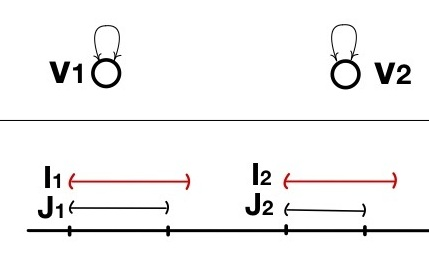
\includegraphics[width=0.4\textwidth]{recursos/capturas/Dgrf_Int_Adj01.jpg}
  \caption{Digráfica de intervalos ajustada. Dos vértices y sin flechas salvo lazos.}
  \label{fig:DgrfAdj01}
\end{figure}

En el segundo ejemplo, se puede encontrar nuevamente una representación por pares de intervalos que satisfaga el ajuste planteado por Tomás Feder et al. 

\begin{figure}[H]
  \centering
  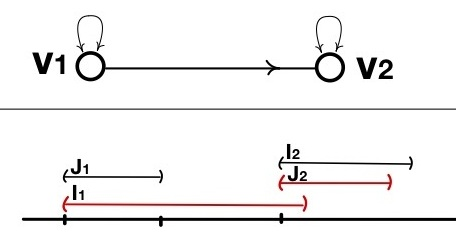
\includegraphics[width=0.45\textwidth]{recursos/capturas/Dgrf_Int_Adj02.jpg}
  \caption{Digráfica de intervalos ajustada. Dos vértices, una flecha.}
  \label{fig:DgrfAdj02}
\end{figure}

Finalmente, si agregamos la flecha $(v_2, v_1)$ entonces damos la siguiente representación ajustada por pares de intervalos. 

\begin{figure}[H]
  \centering
  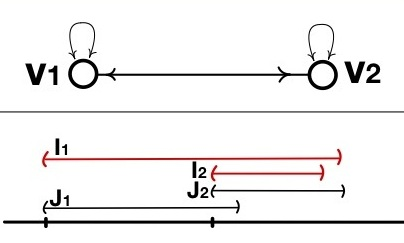
\includegraphics[width=0.4\textwidth]{recursos/capturas/Dgrf_Int_Adj03.jpg}
  \caption{Digráfica de intervalos ajustada con dos vértices y dos flechas.}
  \label{fig:DgrfAdj03}
\end{figure}

A continuación introducimos definiciones muy sencillas. Dado un camino $P=x_0,\dots,x_n$ en una digráfica $G$ y $u,v \in V(G)$ tales que constituyan una flecha, es decir $(u,v) \in E(G)$ o $(v,u) \in E(G)$ decimos que  $(u,v)$ es una flecha derecha si $(u,v) \in E(G)$ y decimos que es una flecha al revés si $(v,u) \in E(G)$. En \cref{fig:DgrfAdj02} podemos decir entonces que $(v_1,v_2)$ es una flecha derecha porque precisamente $(v_1,v_2) \in E(G)$. De forma similar, $(v_2,v_1)$ es una flecha al revés. Sin embargo, uno ve \cref{fig:DgrfAdj03} y se pregunta qué pasa respecto a $(v_1,v_2)$, a estas flechas las cuales sean tanto derechas como al revés, las llamaremos flechas dobles. Aquellas flechas que no son dobles, como la que se muestra en \cref{fig:DgrfAdj02}, se pueden llamar flechas únicamente derechas o únicamente al revés, según sea el caso. Naturalmente los lazos al ser flechas derechas y al revés, son flechas dobles. Si $(u,v)\in E(G)$ diremos que $u$ domina a $v$ o que $v$ es dominado por $u$, sin importar si $(u,v)$ es una flecha doble o única. Esto llevado nuevamente a \cref{fig:DgrfAdj02}, podemos decir entonces que $v_1$ domina a $v_2$. Estas definiciones nos permiten introducir el concepto de caminos congruentes. Dos caminos $P=x_0, \dots, x_n$ y $Q=y_0, \dots, y_n$ en $G$ se dice que son congruentes si tienen el mismo patrón de flechas derechas y al revés, esto es $P,Q$ son caminos congruentes si y solo si $( x_i,x_{i+1})$ es flecha derecha si y solo si $(y_i, y_{i+1})$ es flecha derecha, para toda $0\leq i \leq n-1 $.

\begin{figure}[H]
  \centering
  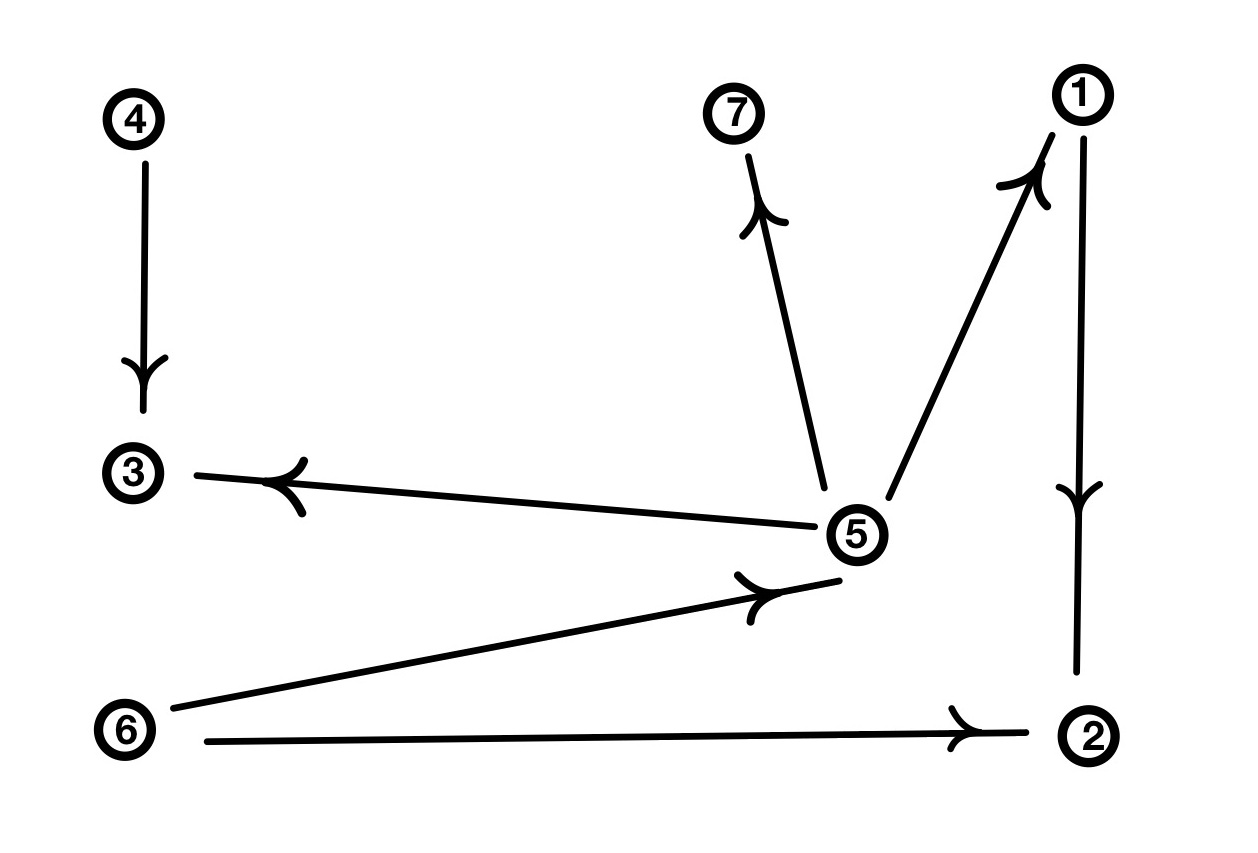
\includegraphics[width=0.4\textwidth]{recursos/capturas/CaminoCngrnt.jpg}
  \caption{Caminos $P=(1,2,6,5,7)$ y $Q=(4,3,5,1,2)$ congruentes.}
  \label{fig:CaminoCngrnt}
\end{figure}

En \cref{fig:CaminoCngrnt} se puede observar un par de camino congruentes $P=(1,2,6,5,7)$ y $Q=(4,3,5,1,2)$. Ahora introducimos una siguiente definición, dados un par de caminos congruentes $P$ y $Q$, decimos que $P$ evita a $Q$ si y solo si no hay flechas $(x_i,y_{i+1})$ en la misma orientación que las flechas $(x_i,x_{i+1})$. En el ejemplo anterior podemos afirmar que $P$ evita a $Q$, sin embargo, $Q$ no evita a $P$, ya que la flecha $(5,1)$ es derecha y la flecha $(5,5)$ al ser una flecha doble en particular es derecha y luego, $Q$ no evita a $P$.

\begin{figure}[H]
  \centering
  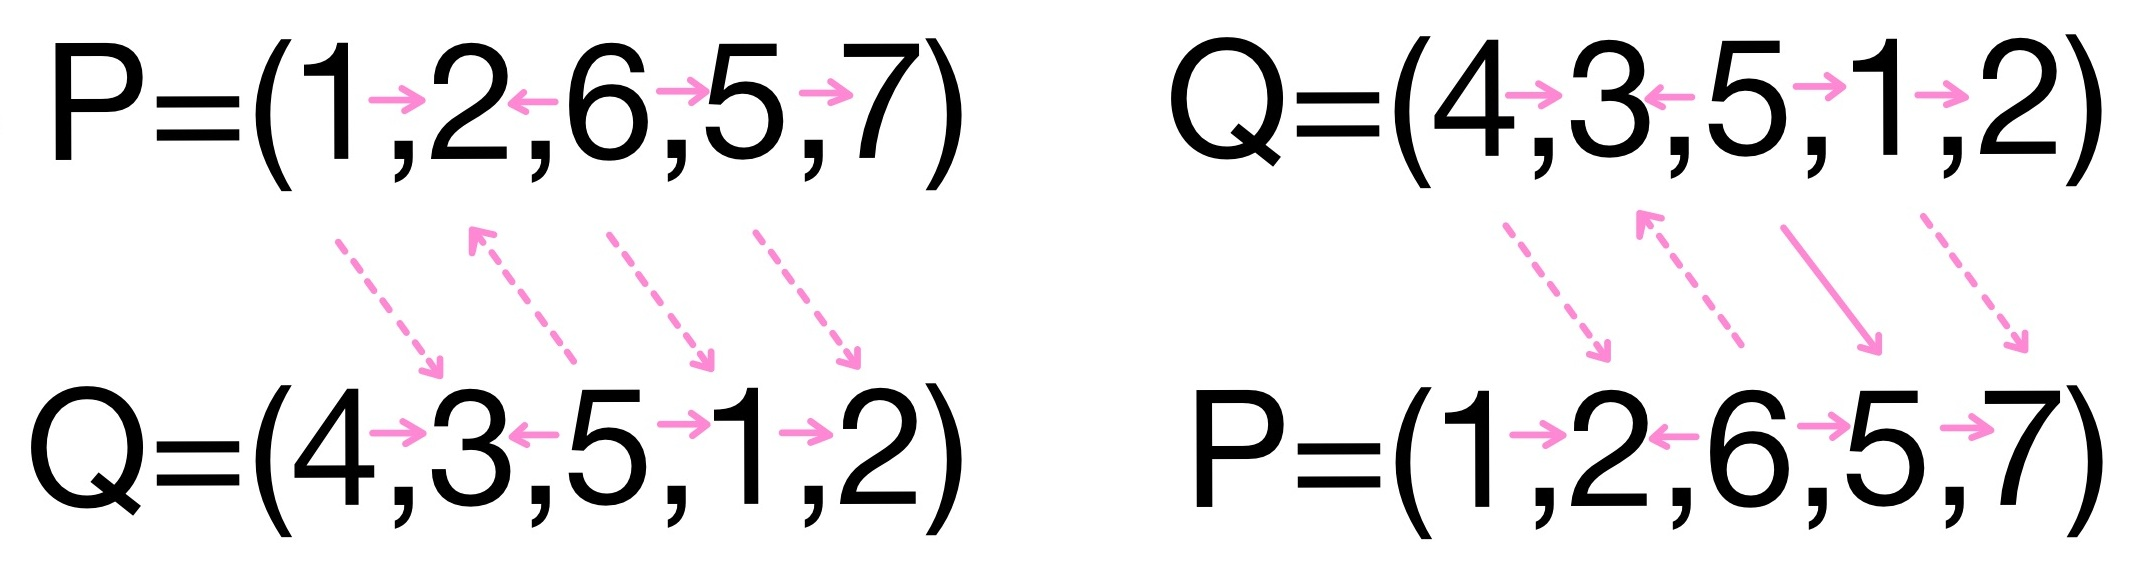
\includegraphics[width=0.5\textwidth]{recursos/capturas/Esqm.jpg}
  \caption{En este esquema las lineas punteadas son flechas que no pertenecen a $E(G)$, así a la izquierda se observa que $P$ evita a $Q$, a la derecha al se verifica que $Q$ no evita a $P$.}
  \label{fig:Esqm}
\end{figure}

Con todo lo anterior podemos dar paso a la definición de \indice{par invertible}, estructura la cual nos permitirá caracterizar a las digráficas de intervalos ajustadas. Un par invertible en una digráfica $G$ es un par de vértices $u,v \in V(G)$ tales que cumplen, en primer lugar, que existen caminos congruentes $P$ de $u$ a $v$ y $Q$ de $v$ a $u$ de tal forma que $P$ evita a $Q$, y en segundo lugar, que existen caminos congruentes $P'$ de $v$ a $u$ y $Q'$ de $u$ a $v$, de tal forma que $P'$ evita a $Q'$.

A continuación damos un par de ejemplos de digráficas que tienen pares invertibles. Para nuestro primer ejemplo damos el $4$-ciclo $(1,2,3,4,1)$. Afirmamos que en esta digráfica los vértices $1$ y $3$ constituyen nuestro par invertible. Para esto damos los caminos congruentes $P=(1,2,3), Q=(3,4,1)$, notemos que así definidos los caminos son congruentes, tal y como se ilustra en el esquema de la derecha del $4$-ciclo de \cref{fig:InvrtblPair01} y además $P$ evita a $Q$ (las flechas en gris no pertenecen a $E(G)$). Recordando nuestra definición, necesitamos ahora otro par de caminos congruentes $P'$ y $Q'$, estos los definimos de la siguiente manera $P'=(3,2,1), Q'=(1,4,3)$ nuevamente usando el esquema de \cref{fig:InvrtblPair01}, se comprueba que dichos caminos son congruentes y que además $P'$ evita a $Q'$.

\begin{figure}[H]
  \centering
  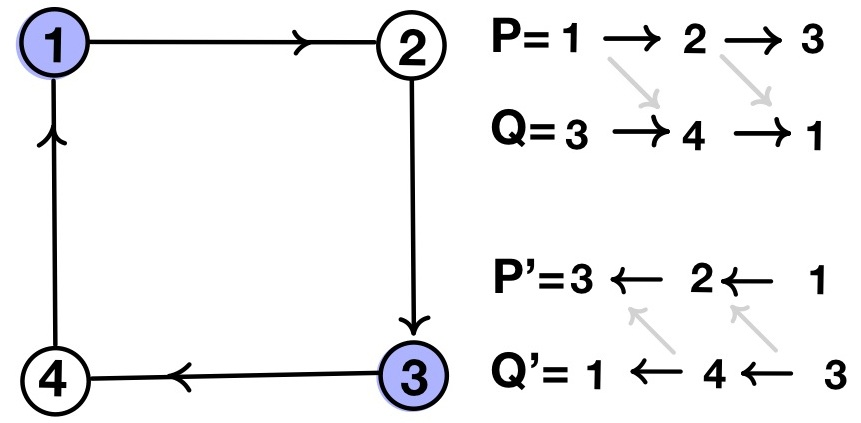
\includegraphics[width=0.5\textwidth]{recursos/capturas/InvtblPair01.jpg}
  \caption{Los vértices azules constituyen un par invertible. A la derecha los caminos congruentes $P,Q$, $P',Q'$.}
  \label{fig:InvrtblPair01}
\end{figure}

Un hecho interesante del ejemplo anterior es que es posible definir a $P'$ y a $Q'$ como los caminos inversos de $P$ y $Q$ respectivamente, donde entendemos que dado un camino $(x_0,x_1, \dots, x_n)$ el camino inverso es $(x_n,x_{n-1}, \dots, x_0)$. Aunque esto no se puede hacer en general, en este caso, la validez de lo anterior se debe a que tanto $P$ evita a $Q$ como $Q$ evita a $P$. 

A continuación hacemos simétricas las flechas de la gráfica anterior para tener un ejemplo donde es imposible definir a $P', Q'$ como los caminos inversos de $P, Q$ respectivamente. Veamos \cref{fig:InvrtblPair02}. Nuevamente tenemos que los vértices $1$ y $3$ son un par invertible. Algo importante a destacar es que los pares de caminos del ejemplo pasado, si bien siguen siendo congruentes, dejan de evitarse. Por ejemplo para que $P$ evite a $Q$ necesitamos que $(1,4),(2,1)\notin E(G)$, algo que no sucede en el presente ejemplo. Por lo anterior es necesario dar otro par de caminos $P$ y $Q$. Definimos $P=(1,2,2,3,3)$ y $Q=(3,3,4,4,1)$. Así definidos los caminos, son congruentes y además $P$ evita a $Q$. Si uno tratara de definir los caminos $P'$ y $Q'$ como los caminos inversos de $P$ y $Q$ respectivamente, uno caería en cuenta que así definidos el camino $P'$ no evita a $Q'$. Por lo que debemos encontrar otra forma alterna para definir a $P'$ y a $Q'$. Así, damos $P'=(3,4,4,1,1)$ y $Q'=(1,1,2,2,3)$ y definidos de esta forma, $P', Q'$ son caminos congruentes y son tales que $P'$ evita a $Q'$.

\begin{figure}[H]
  \centering
  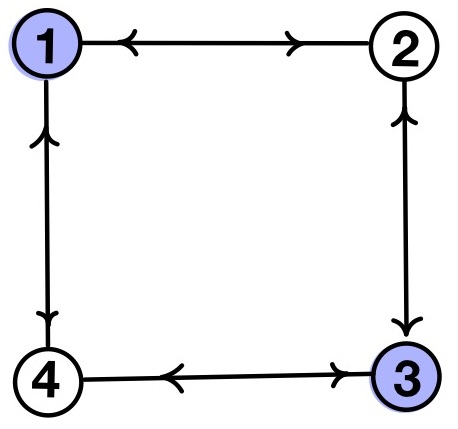
\includegraphics[width=0.5\textwidth]{recursos/capturas/InvrtblPair02.jpg}
  \caption{Los vértices azules constituyen un par invertible.}
  \label{fig:InvrtblPair02}
\end{figure}

En los ejemplos pasados se puede verificar mediante argumentos simétricos que los vértices $2,4$ son también pares invertibles. 

A continuación definiremos una digráfica auxiliar, en la cual se rescata bastante información respecto a todos los pares invertible de una gráfica $G$, en caso de que existan. Dada una digráfica $G$, definimos la digráfica de pares asociada a $G$, denotada por $G^{+}$ la cual está definida como $V(G^{+})=\{ (u,v)\in G\times G \colon\ u\neq v \}$ y diremos que $((u,v),(u',v'))\in F(G^{+})$ si y solo si sucede una de las siguientes dos cosas; $(u,u'),(v,v')\in E(G)$ y $(u,v')\notin E(G)$ o si sucede que $(u',u),(v',v)\in E(G)$ y $(v',u)\notin E(G)$. Usemos como ejemplo \cref{fig:InvrtblPair01} para dar la digráfica de pares asociada.

\begin{figure}[H]
  \centering
  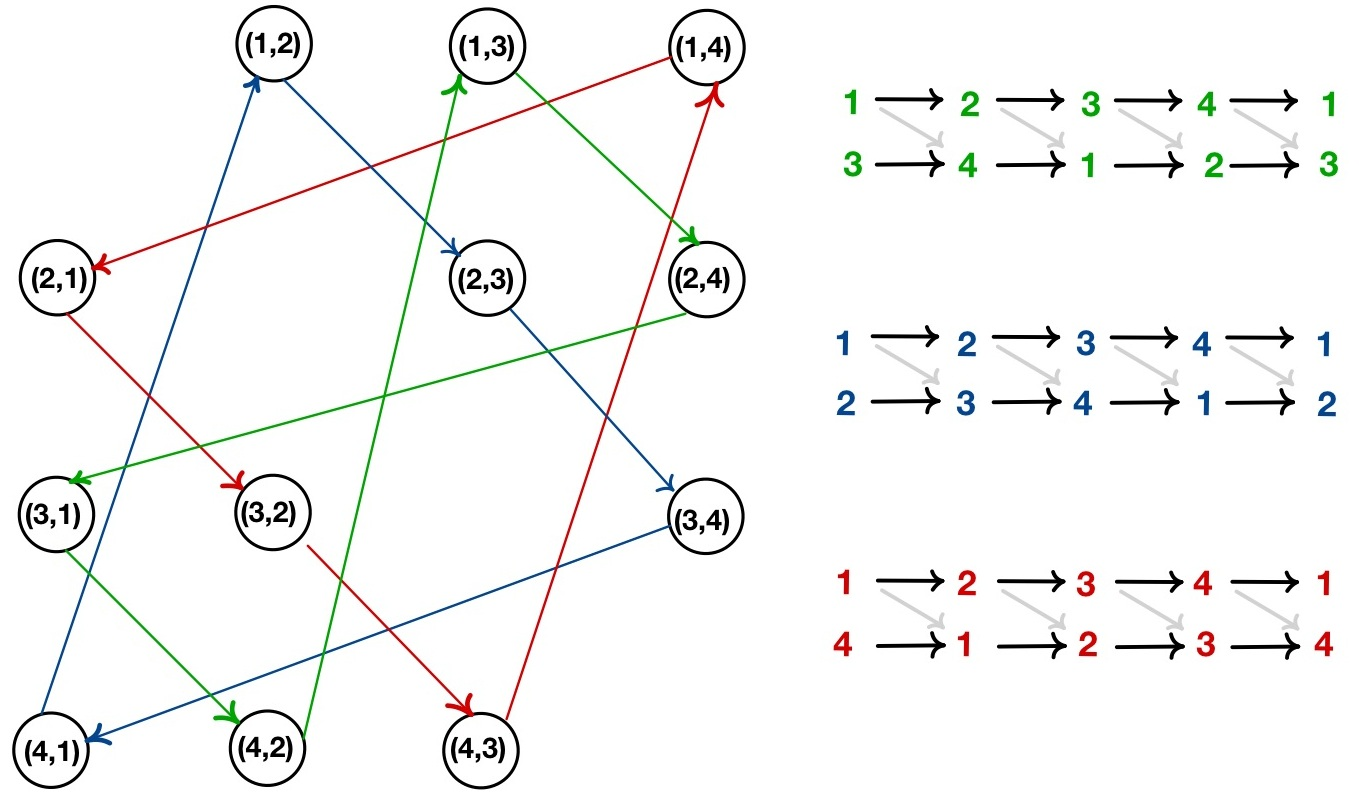
\includegraphics[width=0.75\textwidth]{recursos/capturas/PairDgrph.jpg}
  \caption{Los colores distintos corresponden a las componentes fuertes de $G^+$.}
  \label{fig:InvrtblPair02}
\end{figure}

Apoyándonos del esquema de la derecha, podemos verificar que en efecto las flechas que están dibujadas, son flechas según la definición de las flechas de la digráfica de pares. Coloreamos de colores distintos las tres componentes fuertes distintas. Como hicimos notar, la pareja de vértices $2,4$ también constituye un par invertible, algo interesante es el hecho que los vértices $(1,3)$ y  $(2,4)$ pertenecen a la misma componente fuerte (verde). El siguiente teorema nos dice más sobre esta interesante observación y también arroja más información sobre el resto de vértices y las componentes conexas.

\begin{teorema}
\label{teo:PairDigrph}
    Supongamos que $u$ y $v$ forman un par invertible de la digráfica $G$. Entonces $(u,v)$ y $(v,u)$ pertenecen a la misma componente fuertemente conexa $C$ de la digráfica de pares $G^+$. Más aún, cualquier otra pareja $(x,y)$ que pertenezca a $C$, cumple que su par revertido $(y,x)$ es también elemento de $C$.  Como consecuencia, si $(x,y) \in C$ entonces $x,y$ es un par invertible. Por otro lado si $H$ no tiene pares invertibles, entonces por cada componente fuerte $C$ de $G^+$, existe una componente fuerte $C' \neq C$ tal que $(x,y)\in C $ si y solo si $(y,x)\in C'$
\end{teorema}


Antes de continuar con la prueba veremos otra cosa interesante que sucede en la digráfica de pares $G^+$. Si tenemos que en $G^+$ hay un camino \textbf{P} de $(u,v)$ a $(v,u)$ digamos \textbf{P}$=( (u,v), (x_1,y_1), \dots, (x_{n},y_n), (v,u)) $ entonces en automático tendremos un par de caminos $P,Q$ congruentes, $P=(u, x_1, \dots, x_n,v)$ de $u$ a $v$ y $Q=(v,y_1, \dots, y_n, u)$ de $v$ a $u$ y que además $P$ evita a $Q$. De donde $P$ y $Q$ se obtienen al considerar solo las primeras entradas del camino \textbf{P} y al considerar solamente las segundas entradas del camino \textbf{P}, respectivamente.
Análogamente, si también existe un camino en $G^+$ de $(v,u)$ a $(u,v)$, tendremos que existen otro par de caminos $P',Q'$ congruentes, $P'$ de $v$ a $u$ y $Q'$ de $u$ a $v$ tales que $P'$ evita a $Q'$. Donde $P', Q'$ se construirán de forma similar a como se construyeron $P$ y $Q$. Así, en el caso en el que hay un camino \textbf{P} de $(u,v)$ a $(v,u)$ en $G^+$ y otro camino \textbf{Q} de $(v,u)$ a $(u,v)$ en $G^+$, podremos afirmar que $u,v$ constituyen un par invertible de $G$. 

\begin{proof}
    Probemos como primer punto que si $u,v$ son un par invertible, entonces $(u,v)$ y $(v,u)$ pertenecen a la misma componente fuertemente conexa.
    Ahora veamos que si $(x,y)\in C$ entonces $(y,x)\in C$. Para esto haremos una primera nota, $((u,v),(u',v'))\in E(G^+)$ implica que $((v',u'),(v,u))\in E(G^+)$, esto se puede corroborar observando \cref{fig:FlechaRevertida}. Ahora sí, continuemos con la prueba, como $(x,y) \in C$ entonces la reversa de un camino cerrado que contiene a $(u,v),(x,y)$ (usando la observación) es un camino cerrado que contiene a $(v,u),(y,x)$.    Luego, por concatenación de estos caminos cerrados, obtenemos otro camino cerrado que contiene a $(u,v),(v,u)$ y así podemos concluir que $(x,y),(y,x)$ pertenecen a la misma componente fuerte $C$. Esto se puede observar en \cref{fig:RvrtdPath}. 
    Finalmente si no existe un par invertible, para cada $(x,y)$ sabemos que $(y,x)$ no pertenece a la misma componente de $(x,y)$ pues en ese caso $x,y$ en efecto constituye un par invertible. Luego para cada $(x,y)\in C$ existe una componente $C'$ tal que $(y,x)\in C'$. 
\end{proof}

\begin{figure}[H]
  \centering
  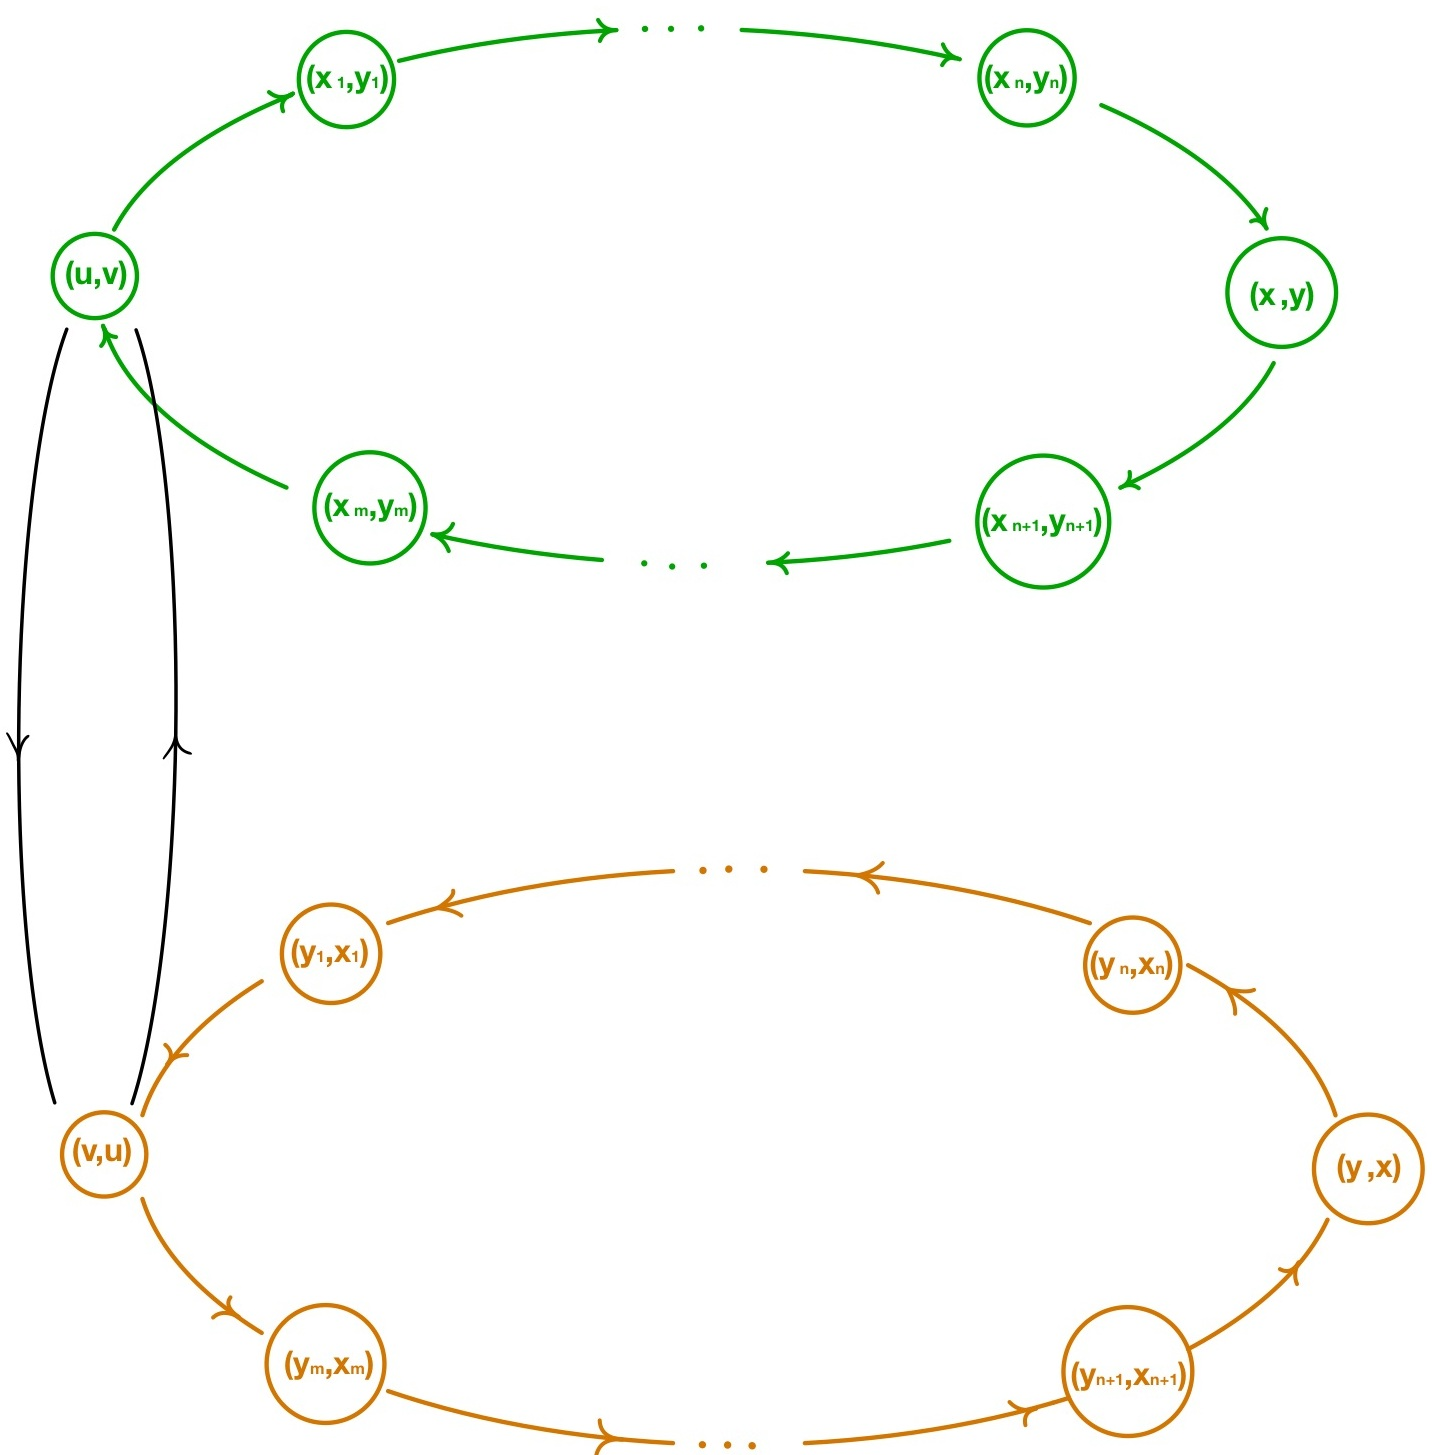
\includegraphics[width=0.65\textwidth]{recursos/capturas/RvrtdPath.jpg}
  \caption{En verde el camino cerrado que contiene a $(u,v),(x,y)$. En naranja el camino revertido del camino verde. Al seguir el sentido de las flechas se obtiene un camino que contiene a $(uv),(v,u)$ }
  \label{fig:RvrtdPath}
\end{figure}

\begin{figure}[H]
  \centering
  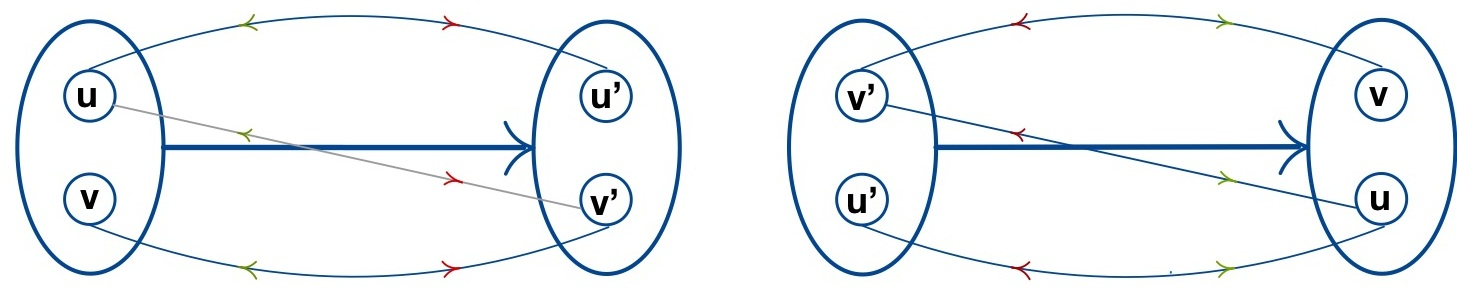
\includegraphics[width=0.85\textwidth]{recursos/capturas/(uv,u'v').jpg}
  \caption{Si $(uv,u'v')\in E(G^+)$ entonces $(v'u',vu)\in E(G^+)$. Representamos en color verde y rojo las flechas de los dos casos distintos que se obtiene cuando $(uv,u'v')\in E(G^+)$. En color gris representamos una flecha que no pertenece a $E(G)$.}
  \label{fig:FlechaRevertida}
\end{figure}

En el siguiente teorema, exhibimos un nuevo concepto, el de ordenamiento mínimo. Más adelante veremos que este concepto esta íntimamente relacionado con las digráficas de intervalos ajustadas, mas aún mostramos un pequeño algoritmo para dada una digráfica de intervalos ajustada construir un ordenamiento mínimo o dado un ordenamiento mínimo de una digráfica de intervalos ajustada, construir un representación por pares de intervalos de la digráfica.

\begin{teorema}
\label{teo:OrdLnl}
    Sea $G$ una digráfica reflexiva, entonces un orden lineal $<$ es un ordenamiento m\'inimo si y solo si, para cualesquiera tres vértices $i<j<k$ tenemos que \textbf{}
    $$ik\in E(G) \text{ implica } ij\in E(G)$$
    $$ki\in E(G) \text{ implica } ji\in E(G)$$
\end{teorema}
\begin{proof}
    Supongamos que $<$ es un ordenamiento m\'inimo, entonces $ab,jj\in E(G)$. Luego $\min(a,j) \min(b,j)\in E(G)$, donde $a,b \in \{ i,k\}$ con $a \neq b$.
    Ahora dados $xy, x'y' \in E(G)$ veamos que $\min(x,x') \min(y,y')\in E(G)$. Todos los posibles casos son los siguientes:
    
    $ i) x<x' $ y $ y<y' $ \hspace{1cm} $iii) x<x' $ y $ y'<y $
    
    $ ii) x'<x $ y $ y'<y $ \hspace{1cm} $iv) x'<x $ y $ y<y' $

    De los dos primeros dos casos se concluye fácilmente que $\min(x,x') \min(y,y')\in E(G)$ pues:
    $$x<x' \text{ y } y<y' \Rightarrow \min(x,x') \min(y,y')=xy \text{ y } xy\in E(G) \text{por hipótesis.}$$
    $$x'<x \text{ y } y'<y \Rightarrow \min(x,x') \min(y,y')=x'y' \text{ y } x'y'\in E(G) \text{por hipótesis.}$$
    
    Los casos iii) y iv) hay que tratarlos de otra forma, probaremos solo iii) pues iv) es totalmente análogo.
    Tenemos que $x<x' $ y $ y'<y\Rightarrow \min(x,x') \min(y,y')=xy' $ En este punto se nos presentan los siguientes casos; $x=y$ luego dado que $H$ es reflexiva, el lazo $xy\in E(G)$, el segundo caso $x<y' $. Como $y'<y$ obtenemos la cadena de desigualdades $x<y'<y$ y como $xy\in E(G)$ entonces $xy'\in E(G)$, como tercer y último caso, tenemos que $y'<x$. Entonces $x<x'$ así $y'<x<x'$ y $x'y'\in E(G)$ luego $xy'\in E(G)$. En cualquiera de los dos casos anteriores se tiene que $min(x,x')min(y,y')\in E(G)$. Por lo que podemos concluir que en efecto $<$ es un ordenamiento mínimo.
\end{proof}

A partir del teorema anterior podemos obtener el siguiente corolario.

\begin{corolario}
\label{cor:Orden_Flechas}
    Sea $G$ una digráfica reflexiva. Un ordenamiento lineal de los vértices de $G$ es un ordenamiento mínimo si y solo si para cada vértice $v$, los vértices que siguen a $v$ en el orden, consisten de: i) Primero aparecen (en el orden) los vértices que son adyacentes a $v$ por flechas simétricas. ii) En segundo lugar aparecen los vértices que son adyacentes a v por aristas asimétricas, además son todas derechas o todas izquierdas, iii) Finalmente tenemos vértices que no tinen flechas desde o hacia $v$
\end{corolario}

\begin{proof}
    Esto es fácil de verificar, supongamos que $u<v<w$ y supongamos que $uw,wu\in E(G)$ veremos que si esto pasa por fuerza $v$ debe tener también flechas dobles hacia $u$, es decir, no puede tener flechas asimétricas ni puede no tener flechas desde o hacia $u$.
    Por la primera consecuencia de \cref{teo:OrdLnl} se tiene que $uv\in E(G)$, y por la segunda consecuencia, tenemos que $vu\in E(G)$. Así $v$ debe tener flechas simétricas hacia $u$. 
    Verifiquemos rápidamente que si $u<v<w$ y hay una flecha asimétrica de $u$ a $w$, entonces debe haber una flecha asimétrica con la misma dirección de $u$ a $v$. Nuevamente el resultado es bastante inmediato del \cref{teo:OrdLnl}, ya que si $uw\in E(G)$ entonces $uv\in E(G)$ o análogamente si $wu\in E(G)$ entonces $vu\in E(G)$.
\end{proof}

\begin{teorema}
    \label{teo:DigrfIntAdj_OrdMin}
    Una digráfica reflexiva es una digráfica de intervalos ajustada si y solo si admite un ordenamiento mínimo.
\end{teorema}

\begin{proof}
    Comencemos probando que si $G$ es una digráfica de intervalos ajustada entonces admite un ordenamineto mínimo de sus vértices. Para esto definimos $u<v$ si y solo si el extremo izquierdo de $I_u$ es menor que el extremo izquierdo de $I_v$. Esto corresponde a un ordenamiento mínimo de los vértices de $G$.  
    Ahora, dado un ordenamiento mínimo de una digráfica reflexiva $G$, podemos ordenar los puntos iniciales de $I_v$ y de $J_v$ en el mismo orden en los cuales aparecen los vértices $v\in V(G)$ respecto al ordenamiento mínimo y definimos los intervalos $I_v$ y $J_v$ como: el intervalo $I_v$ termina en en el punto correspondiente al último vértice $w$ tal que $vw$ es una flecha derecha y el intervalo $J_v$ termina en el punto correspondiente al último vértice tal que $vw$ es un vértice es una flecha al revés.
\end{proof}

En \cref{fig:MinOrdToIntGrph}, observamos una digráfica reflexiva $G$ la cual admite un ordenamiento mínimo, definido precisamente por el orden natural de su etiqueta, es decir $1<2< \cdots <7$. Es fácil verificar mediante \cref{cor:Orden_Flechas} que este es en efecto un ordenamiento mínimo. Por ejemplo para el vértice $1$ tenemos que en el orden primero aparecen los vértices $1,2$ que tienen flechas dobles, luego aparecen los vértices $4,5$ que tienen flechas derechas y finalmente tenemos los vértices $6,7$ que no forman flechas con el vértice $1$. Este análisis se puede extender hacia el resto de los vértices.
Ahora veamos cómo se realiza la construcción de los conjuntos de intervalos $\{I_v\}_{v\in V(G)}, \{J_v\}_{v\in V(G)}$. El algoritmo descrito en la prueba  d\cref{teo:DigrfIntAdj_OrdMin} Nos dice que $I_1, J_1$ empiezan en $1$ e $I_1$ termina en el último vértice $v$ tal que hay una flecha derecha, en este caso $5$ es el último vértice tal que $(1,5)$ es flecha derecha, así $I_1=[1,5]$, tal como se indica a la derecha de \cref{fig:MinOrdToIntGrph}. Ahora $J_1$ termina en el último vértice $v$ tal que $(1,v)$ es flecha al revés. En este caso es el vértice $3$. Un caso curioso es el del vértice $5$, veamos, $I_5,J_5$ ambos deben empezar con $5$ ahora $I_5$ debe terminar en el último vértice $v$ tal que $(5,v)$ es flecha derecha, debemos recordar que al estar en una digráfica reflexiva los lazos son flechas simétricas es decir, son derechas y al revés. Así el extremo derecho de $I_5$ es nuevamente $5$. Finalmente el extremo derecho de $J_5$ también corresponde a $5$. 


\begin{figure}[H]
  \centering
  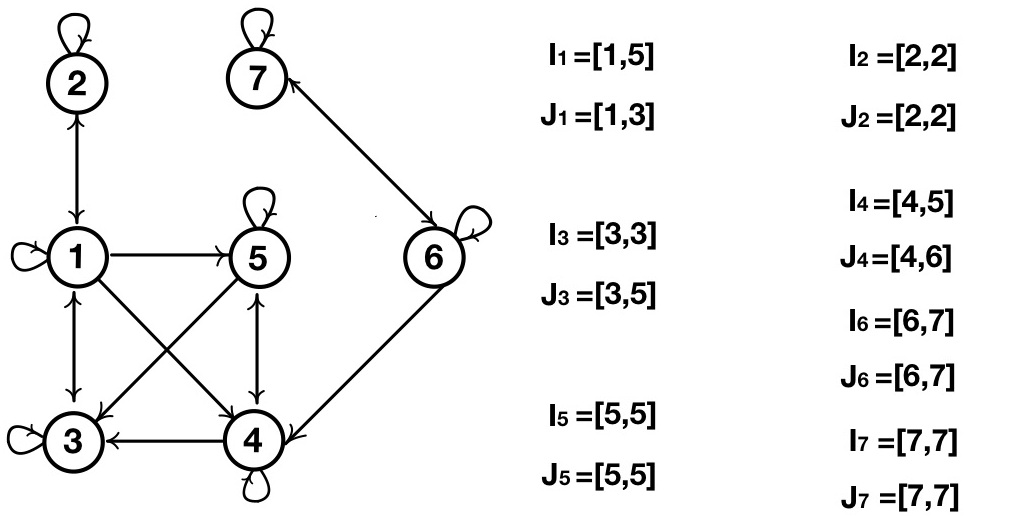
\includegraphics[width=0.75\textwidth]{recursos/capturas/MinOrdToIntGrph.jpg}
  \caption{Dada una digráfica reflexiva $G$ que admite un ordenamiento mínimo construimos la representación por pares de intervalos de $G$.}
  \label{fig:MinOrdToIntGrph}
\end{figure}

\begin{teorema}
    \label{teo:OrnMin_NoInvPair}
    Si $G$ tiene un par invertible, entonces $G$ no tiene un ordenamiento mínimo.
\end{teorema}

\begin{proof}
    Sea $u,v$ un {\color{malva} par invertible} en $G$. Por \cref{teo:PairDigrph} sabemos que $(u,v),(v,u)$ pertenecen a la misma componente conexa de la digráfica de pares $G^+$. 
    Ahora, supongamos que $(x,y)(x', y')$ es una flecha de la digráfica de pares $G^+$. Supongamos que $<$ es un ordenamiento mínimo de $G$ y supongamos que $ u < v$. Entonces también se tiene que $u'< v'$. Hagamos la prueba de este hecho. Como $(u,v)(u',v')\in E(G)$ entonces tenemos una de las siguientes dos situaciones, i) $uu', vv'\in E(G)$ o $uv'\notin E(G) $ o ii) $u'u, v'v \in E(G)$ o $ v'u \notin E(G) $. En el primer caso, veamos vía contradicción que $u'<v'$.  Supongamos que $v'<u'$. Como $(u,v)(u',v')\in E(G)$ entonces $\min \{u,u' \}\min \{v,v' \}\in E(G)$, ya que por hipótesis tenemos un ordenamiento mínimo. Por otro lado, en el caso i) también tenemos la hipótesis $uv'\notin E(G)$, luego $\min \{u,u' \}\min \{v,v' \} \neq uv'$. Por lo que $\min \{u,u' \}=u'$ o $\min \{v,v' \}= v$. En el caso $\min \{u,u' \}=u'$, se tiene la siguiente cadena $v'<u'<u<v$ de donde $v'<u<v$ y dado que $vv'\in E(G)$, entonces por \cref{teo:OrdLnl} se tiene que $uv'\in E(G)$ lo cual es una contradicción. Ahora en el caso en el que $\min \{v,v' \}= v$ se tiene la cadena $u<v<v'<u'$ de donde $u<v'<u'$ y dado que $uu'\in E(G)$ usando nuevamente \cref{teo:OrdLnl} $uv' \in E(G)$ lo cual es nuevamente una contradicción. Ahora en el caso ii) como $u'u, v'v \in E(G)$ entonces $\min \{u',v' \}\min \{u,v \}\in E(G)$, ya que tenemos un ordenamiento mínimo. En este caso también tenemos que $v'u\notin E(G)$ así $\min \{u',v' \}  \min \{u,v \}\neq v'u$. Así las cosas $\min \{u',v' \}=u'$ o $\min \{u,v \}=v$. En el caso en que $\min \{u',v' \}=u'$ se llega a $u'<v'$ que es precisamente lo que buscamos, mientras que el segundo caso $\min \{u,v \}=v$ no es posible, ya que en este caso $v<u$ pero por hipótesis $u<v$. Entonces $u = v$ lo cual no es posible. De todo lo anterior se concluye que $u'<v'$.    
    Retomando la prueba, consideremos $P$ el camino cerrado dirigido que contiene a $(u,v),(v,u)$, siguiéndolo y haciendo uso de la nota anterior se llega a una contradicción del tipo $u<v$ y $v<u$.
    Por lo que no es posible tener un ordenamiento mínimo en $G$ si hay presencia de un par invertible.
\end{proof}

\section{Digráficas de intervalos ajustadas.}

En esta sección enunciamos y probamos el teorema central de la tesis. 

\begin{teorema}
    Una digráfica reflexiva $G$ es una digráfica de intervalos ajustada si y solo si no tiene pares invertibles.
\end{teorema}

El teorema anterior lo probaremos vía las siguientes equivalencias.

 \begin{teorema}
     Sea $G$ una digráfica reflexiva, entonces las siguientes proposiciones son equivalentes.
\begin{enumerate}
  \item $G$ es una digráfica de intervalos ajustada.
  \item $G$ no admite un ordenamiento mínimo.
  \item $G$ no tiene pares invertibles.
  \item Los vértices de $G^+$ admiten una partici\'on en dos conjuntos $D, D'$ tales que:
        \begin{enumerate}
            \item $(x,y)\in D $ si y solo si $ (y,x) \in D$
            \item $(x,y)\in D$ y $(x,y)$ domina a $(x',y')$ en $G^+$ implica que $(x',y')\in D$
            \item $(x,y), (y,z)\in D$ implica que $(x,z)\in D$
        \end{enumerate}
\end{enumerate}

\begin{proof}
    La equivalencia entre las primeras dos proposiciones se probó en \cref{teo:DigrfIntAdj_OrdMin}.
    Por otro lado, mediante un uso de contrapositiva sobre \cref{teo:OrnMin_NoInvPair} se obtiene que la segunda proposición implica la tercera. 
    {\color{malva}Para probar que la cuarta proposición implica la segunda, solo basta definir el ordenamiento $<$ como $u<v$ si y solo $(x,y) \in D$. }
    Finalmente procedamos a probar que la tercer proposición implica la cuarta. Haremos la prueba de forma constructiva, es decir mediante un algoritmo veremos que asumiendo que $G$ es débilmente conexa, si no lo fuera, se puede aplicar el proceso a cada componente débilmente conexa y  suponiendo también que $G$ no tiene pares invertibles, construiremos una partición $\{D,D'\}$ de $V(G^+)$, la cual cumple a),b) y c). 
    Haciendo uso de \cref{teo:PairDigrph} se tiene que para cada componente fuertemente conexa $C$ de $G^+$ existe su componente fuerte revertida $C'$, es decir aquella tal que $(x,y)\in C $ si y solo si $(y,x)\in C'$. A las componentes de esta forma les llamaremos componentes fuertemente conexas acopladas o simplemente componentes acopladas.
    La partición de $V(G^+)$ en $D,D'$ corresponderá en separar cada par de componentes acopladas $C$ y $C'$ de $G^+$. Los vértices correspondientes a una componente $C$ los pondremos en $D$ y los vértices revertidos los colocaremos en la componente $D'$. Al realizar el proceso, deberemos tener cuidado en no crear cadenas circulares, es decir una sucesión de pares $(x_0,x_1)(x_1,x_2),\dots, (x_n,x_0)\in D$, ya que buscamos que se satisfaga c) y la existencia de una cadena así implicaría $(x_0,x_0)\in D$, es decir $(x_0,x_0)\in G^+$ pero por construcción en $G^+$ no hay vértices de este estilo (diagonal). 
    Al comenzar el algoritmo los conjuntos $D$ y $D'$ son vacíos. Decimos que una componente fuerte $C$ de $G^+$ es madura si no existen flechas desde $C$ a otra componente fuerte en $G^+ -D$. Entonces el paso general de nuestro algoritmo consistirá precisamente en colocar una componente fuerte madura $C$ en $D$ y colocar a la componente fuerte acoplada $C' $ en $D'$ ($C'$ no será necesariamente madura, pero si se puede garantizar que no hay flechas desde $G^+ -D$ a $C'$, ver \cref{fig:FlechaRevertida}). 
    Mostraremos que en cada paso del algoritmo, es posible añadir al menos una componente fuerte madura a $D$ sin crear cadenas circulares en $D$
    Los conjuntos $D,D'$ tendrán las siguientes propoiedades, las cuales serán ciertas de forma inicial. No existe ninguna cadena circular en $D$, cada componente fuerte de $H^+$ pertenece enteramente a $D, D'$ o $V(G)-\{D,D' \} $ los pares en $D'$ son precisamente los pares revertidos de los pares en $D$; no hay flechas de $G^+$ desde vértices en $D$ a vértices fuera de $D$ y no hay flechas en $G^+$ desde vértices fuera de $D'$ a un vértice en $D'$. Al final del algoritmo, cada par $(x,y)$ con $x\neq y$ pertenecerá a $D$ o a $D'$ y así el $D$ final no tendrá cadenas circulares, por lo que se cumplirá $4$.
    Probemos que todas las propiedades anteriores se mantienen invariantes durante la ejecución del algoritmo.
    Supongamos por contradicción que el actual $D$ no tiene cadenas circulares pero que al añadir $C$, se crea una cadena en $C\cup D$, digamos $((x_0,x_1),(x_1,x_2),\dots, (x_n,x_0))$ además de esto supongamos que que es la primer vez que se obtiene la cadena durante la ejecución del algoritmo, adicionalmente supongase que no hay cadenas circulares mas cortas. Dado que por hipótesis no hay pares invertibles y que nunca se coloca un par y su par revertido en $D$, se tiene que $n\geq 2$. Con todo lo anterior, al menos un par de la cadena debe pertenecer a $C$ asumamos sin pérdida de generalidad que $(x_n,x_0)\in C$ (otros pares pueden estar también en $C$).
    Bajo todas las condiciones anteriores, tenemos los siguientes dos casos.
    Caso 1.- Supongamos que en $G$ hay al menos una flecha entre los vértices $x_0,x_1,\dots,x_n$, digamos $(x_a,x_b)$. Veamos que esto nos implica que ...
 \end{proof}
        
        
        
        
 \end{teorema}